\section{Результаты измерений}
$\varphi_{0} = 179^{\circ} 56' 37'' \pm 5''$

\begin{tabular}{|l|l|l|}
\hline
    $\lambda,\;\text{нм}$ & 1 порядок, $\pm 5 ''$& -1 порядок, $\pm 5 ''$ \\\hline
    $404{,}7$ & $167^{\circ} 24' 48 ''$ & $192^{\circ} 33' 57 ''$ \\\hline
    $435{,}8$ & $165^{\circ} 45' 43 ''$ & $193^{\circ} 59' 9''$ \\\hline
    $491{,}6$ & $165^{\circ} 37' 33''$ & $194^{\circ} 18' 9''$ \\\hline
    $546{,}1$ & $163^{\circ} 58' 12''$ & $195^{\circ} 46' 25''$ \\\hline
    $577$ & $162^{\circ} 53' 54''$ & $196^{\circ} 42' 49''$ \\\hline
    $579{,}1$ & $163^{\circ} 00' 00''$ & $196^{\circ} 46' 25''$ \\\hline
\end{tabular}


\begin{figure}[ht!]
    \center{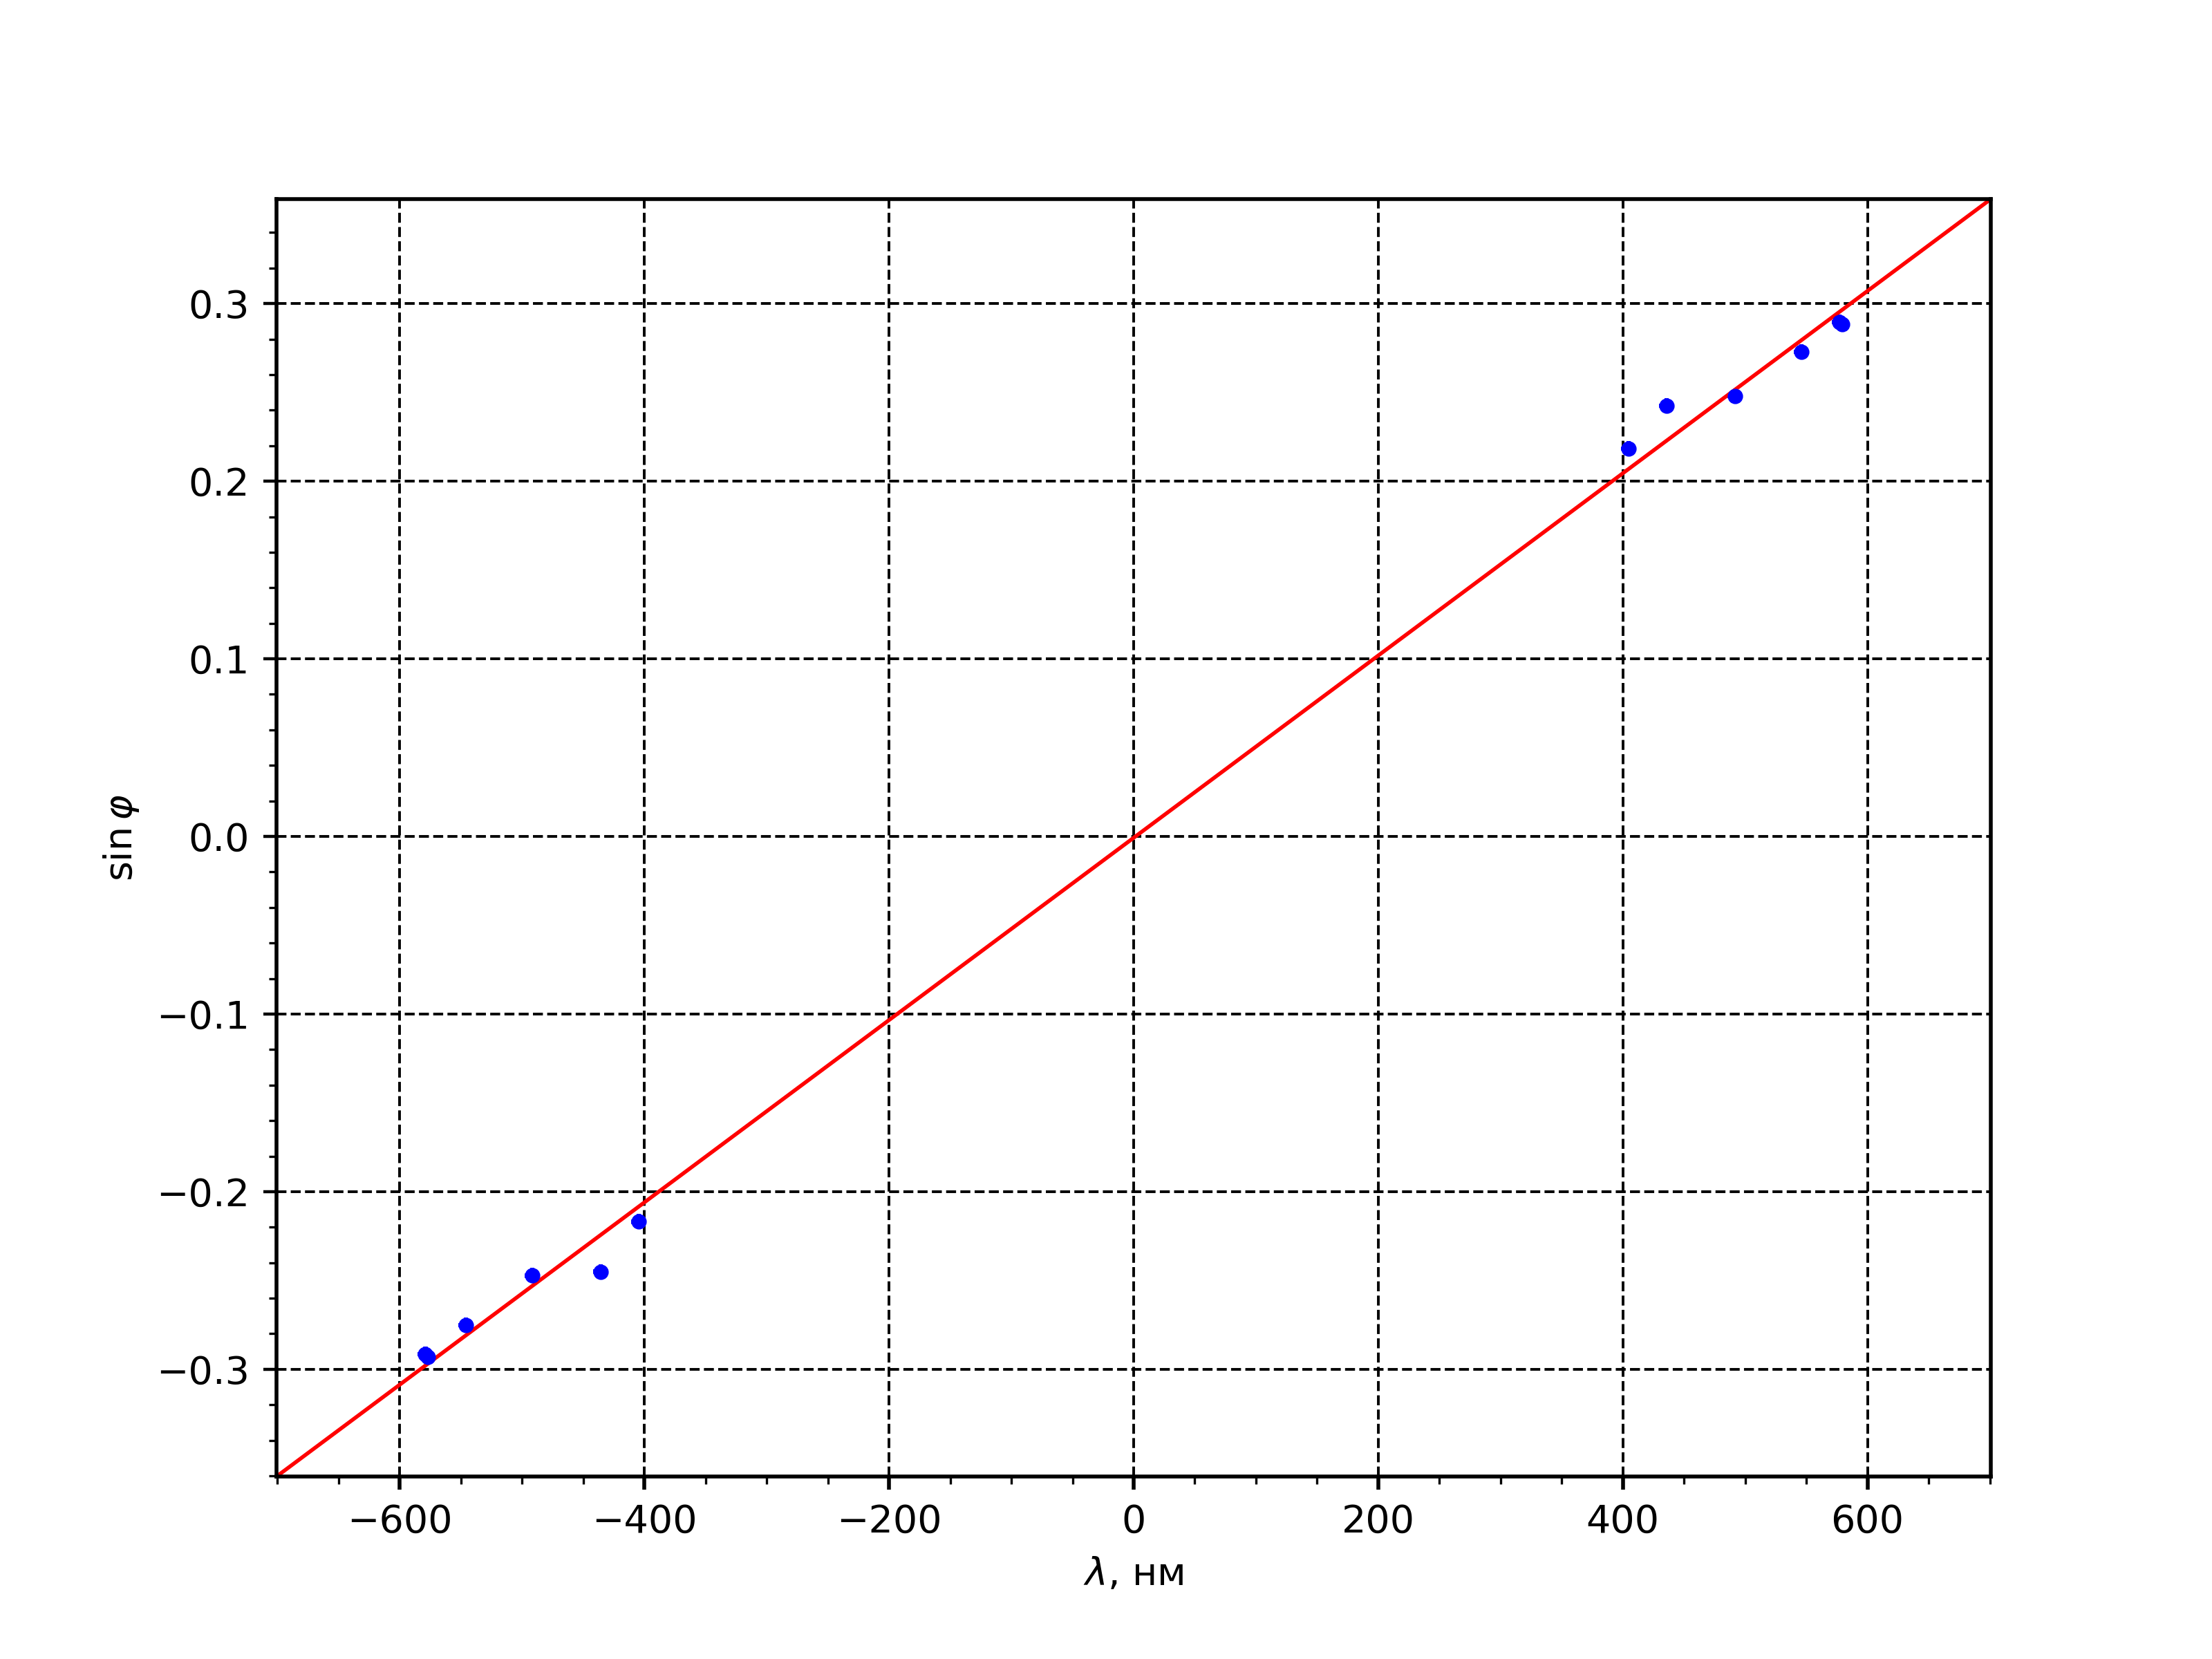
\includegraphics[width=0.8\linewidth]{../img/p1.png}}
\end{figure}

\[
    d = 1{,}95 \pm 0{,}02\;\text{мкм}
\]

Для второго порядка положения линий дуплета $144^{\circ} 38' 35''$ и $144^{\circ} 29' 9''$.

\begin{figure}[ht!]
    \center{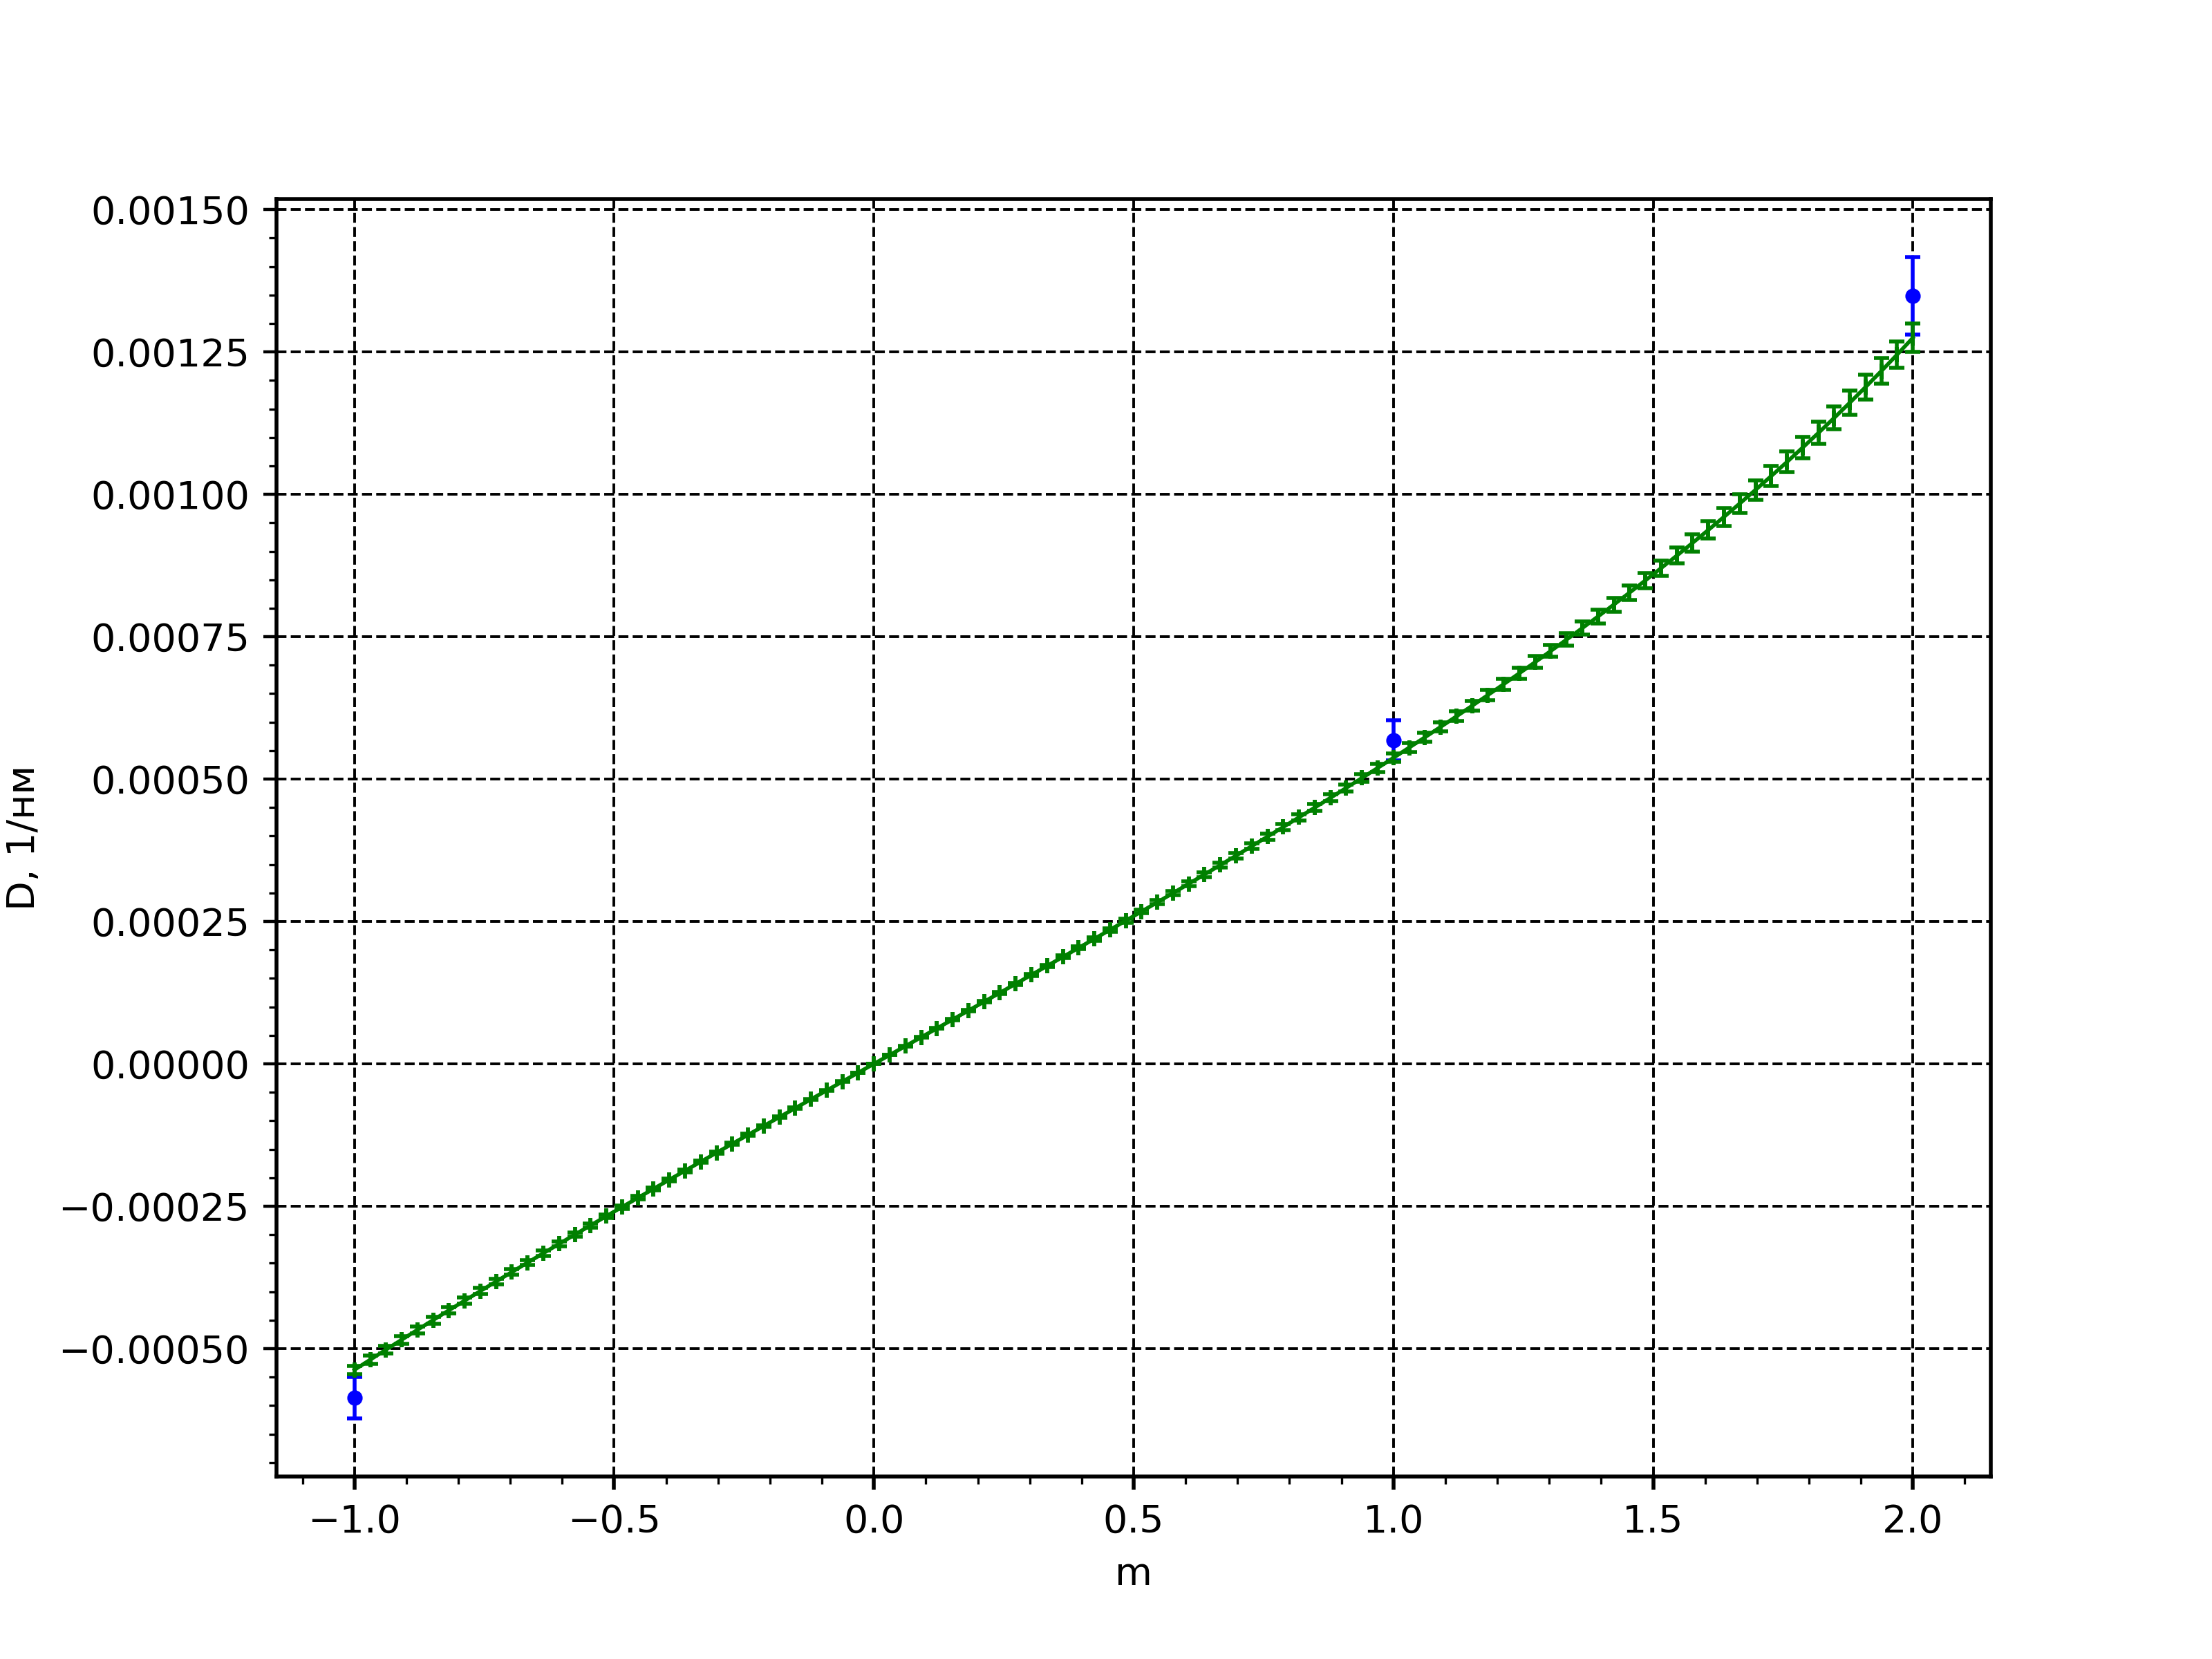
\includegraphics[width=0.8\linewidth]{../img/p2.png}}
\end{figure}

\begin{tabular}{|l|l|l|}
\hline
    порядок & левый край & правый край \\\hline
    -1 & $196^{\circ} 46' 16''$ & $196^{\circ} 45' 13''$ \\\hline
    1 & $162^{\circ} 59' 49''$ & $162^{\circ} 59' 22''$ \\\hline
    2 & $144^{\circ} 29' 33''$ & $144^{\circ} 30' 00''$ \\\hline
\end{tabular}

По 1 порядку
\[
    \delta\lambda = 0{,}26 \pm 0{,}09 \;\text{нм}
\]
\[
    R = \frac{\lambda}{\delta\lambda} = 2000 \pm 700
\]
\[
    n = R / m = R = 2000 \pm 700
\]
\[
    L = nd = 4 \pm 1\;\text{мм}
\]

\newpage
